Comme Python est un langage interprété, on peut l'utiliser de \emph{manière interactive} c'est à dire en écrivant une instruction (ou plusieurs) et en l'exécutant immédiatement. On peut aussi écrire un texte (en respectant une syntaxe particulière) formé d'instructions, l'enregistrer avec un nom de fichier d'\emph{extension} .py  puis exécuter toutes les instructions de contenant.\newline
Sous diverses réserves (en particulier des problèmes de \emph{chemins de dossier} peuvent se produire), cela peut se faire dans n'importe quelle console\footnote{une console est une application dont l'interface avec l'utilisateur est uniquement du texte (ligne de commande).}. Toutefois le programme officiel de la classe nous demande d'utiliser Python par l'intermédiaire d'un \emph{environnement de programation}; au lycée, Spyder a été choisi.\newline
Cet environnement ouvre plusieurs fenêtres (Figure \ref{fig:spyder}) et permet (entre autres) les deux modes d'utilisation.
\begin{itemize}
 \item Dans une fenêtre console/interpréteur, on peut écrire directement une intruction Python et l'exécuter en tapant "Entrée". 
 \item Dans la fenêtre "Editeur de texte" on peut écrire, enregistrer, ... des fichiers d'extension \verb|.py| puis les faire exécuter (bouton Executer du menu ou flèche verte(suivant les versions)) dans une fenêtre console/interpréteur)
\end{itemize}
Dans le dossier "Mes documents", créer un dossier dont le nom vous identifie clairement. Lors d'un TP, vous devrez placer les fichiers que vous créerez dans ce dossier. Notez bien qu'il n'y a aucune sécurité et qu'il peuvent être effacés ou modifiés par n'importe qui. Il est aussi possible que changiez de machine lors d'une autre séance, comme ce dossier n'est pas partagé en réseau, vous n'y accéderez pas. Ce dossier (il sera désigné dans la suite par \emph{dossier de travail}) ne sert donc que temporairement durant une séance de TP. Dans le contexte de la classe, si vous n'utilisez pas une machine personnelle, la sauvegarde la plus commode et sûre se fait par un transfert sur un stockage web en fin de TP.\newline
Exécuter ensuite par l'intermédiaire de Spyder les opérations suivantes.
\begin{enumerate}
 \item Exécuter \verb|1+1| en mode interactif dans une fenêtre d'interpréteur.
 \item Enregistrer un fichier nommé \verb|essai.py| contenant une seule ligne : \verb|1+1| dans votre dossier de travail. Vérifier avec un explorateur de fichier externe qu'il est bien créé. Exécutez le dans un interpréteur de Spyder. 
 
 \begin{figure}[h!]
 \centering
 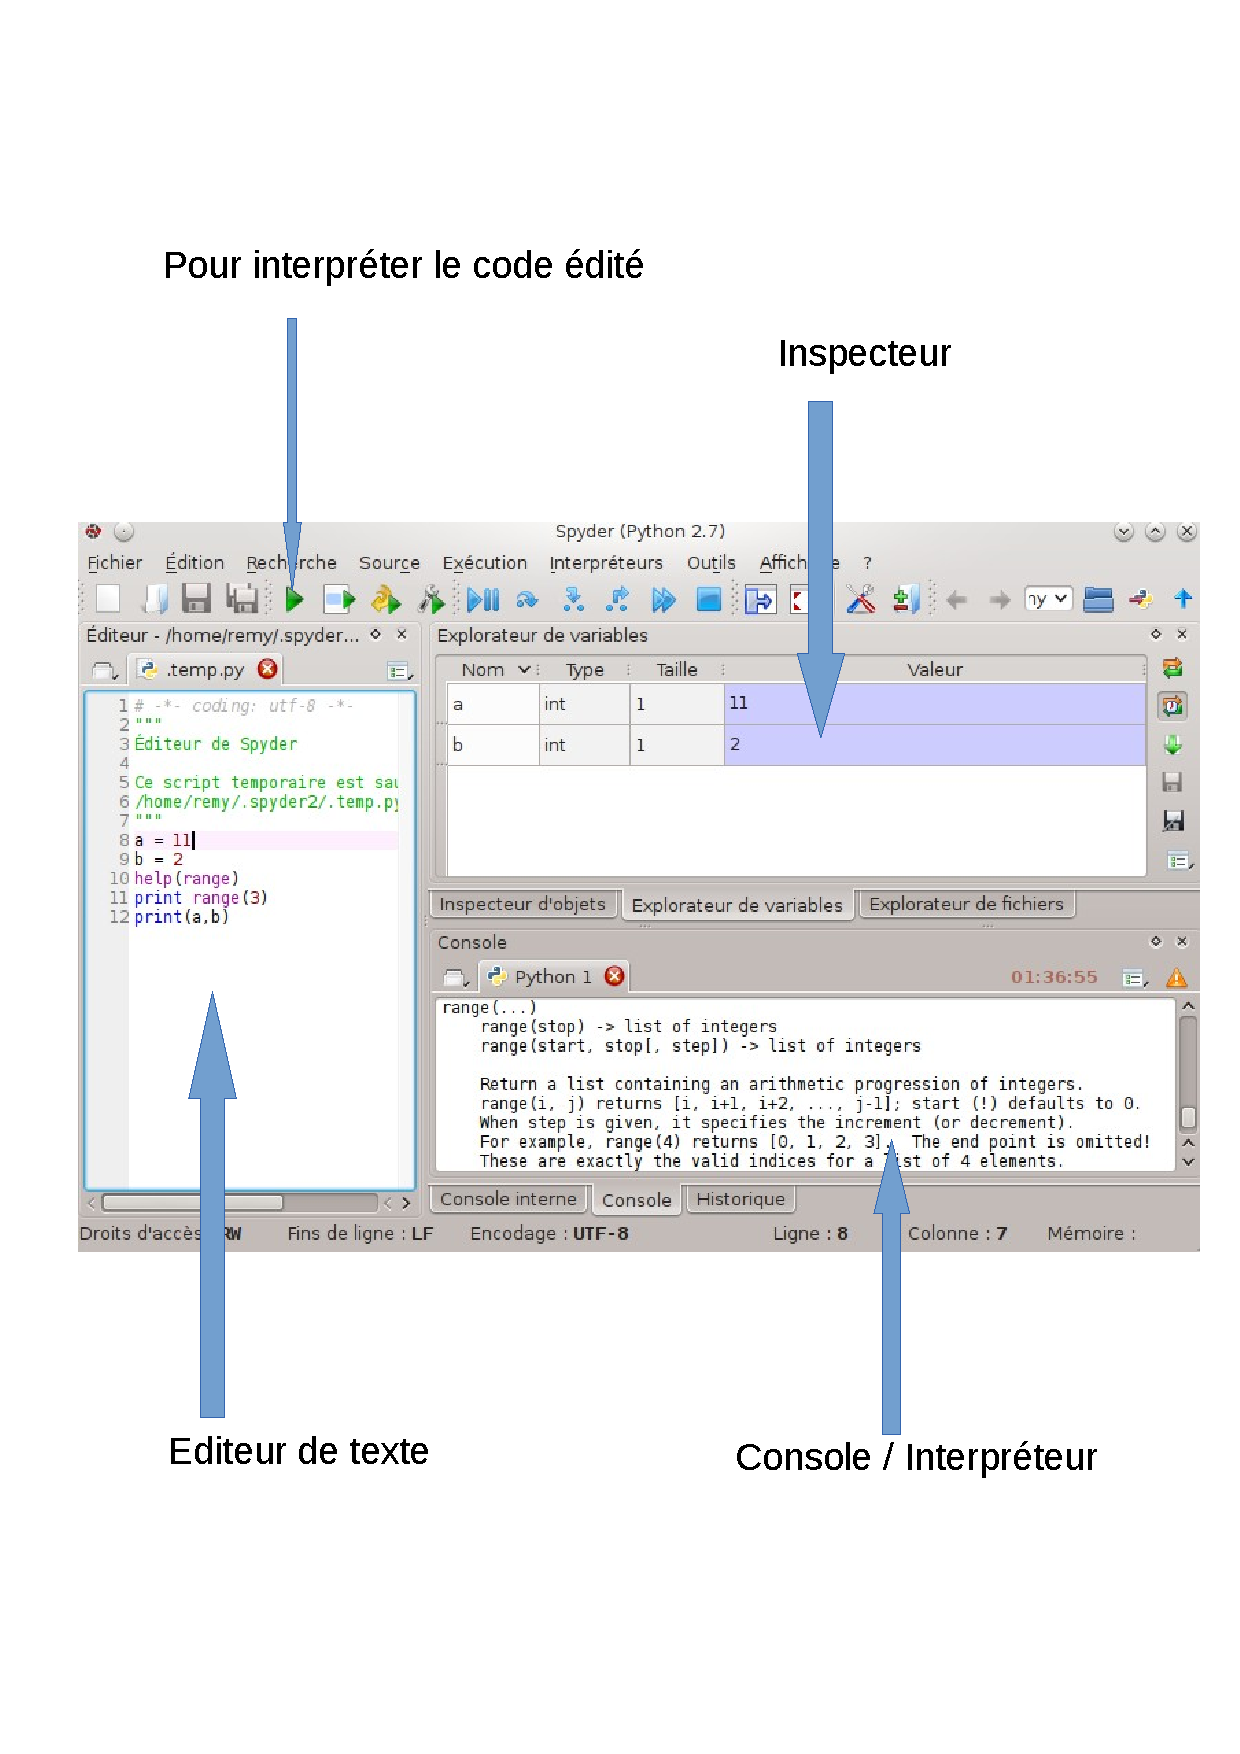
\includegraphics[width=10cm,keepaspectratio=true]{./spyder.pdf}
 % spyder.pdf: 595x842 pixel, 72dpi, 20.99x29.70 cm, bb=0 0 595 842
 \caption{Environnement de développement spyder}
 \label{fig:spyder}
\end{figure}
 \item Ouvrir l'environnement spyder, entrer \verb| print("Hello Word")| dans l'éditeur et interpréter avec la barre d'outils.\newline
 Interpréter directement l'instruction \verb|print("Coucou")| dans la fenêtre.
 \item Dans le coin en haut à droite de la fenêtre de l'interpréteur, repérer le petit triangle jaune avec un point d'exclamation. Il sert à forcer l'arrêt de l'interpréteur lorsqu'il est engagé dans un processus que vous souhaitez stopper. Dans l'éditeur, insérer
 \begin{verbatim}
i = 0
while 0 < 10:
    print('coucou'+str(i))
    i+=1
 \end{verbatim}
\emph{en respectant bien l'indentation} c'est à dire les espaces en début de ligne. Interpréter avec la flèche verte.
\end{enumerate}
On peut citer d'autres environnements, notamment des interpréteurs en ligne: par exemple \href{http://shell.appspot.com}{shell.appspot.com} ou \href{http://live.sympy.org/shellmobile}{live.sympy.org/shellmobile} qui est adapté aux écrans de smartphone et orienté calcul formel  (utilisant le module sympy). 